\documentclass{standalone}
\usepackage{tikz}
\usetikzlibrary{chains, fit, positioning}

\begin{document}
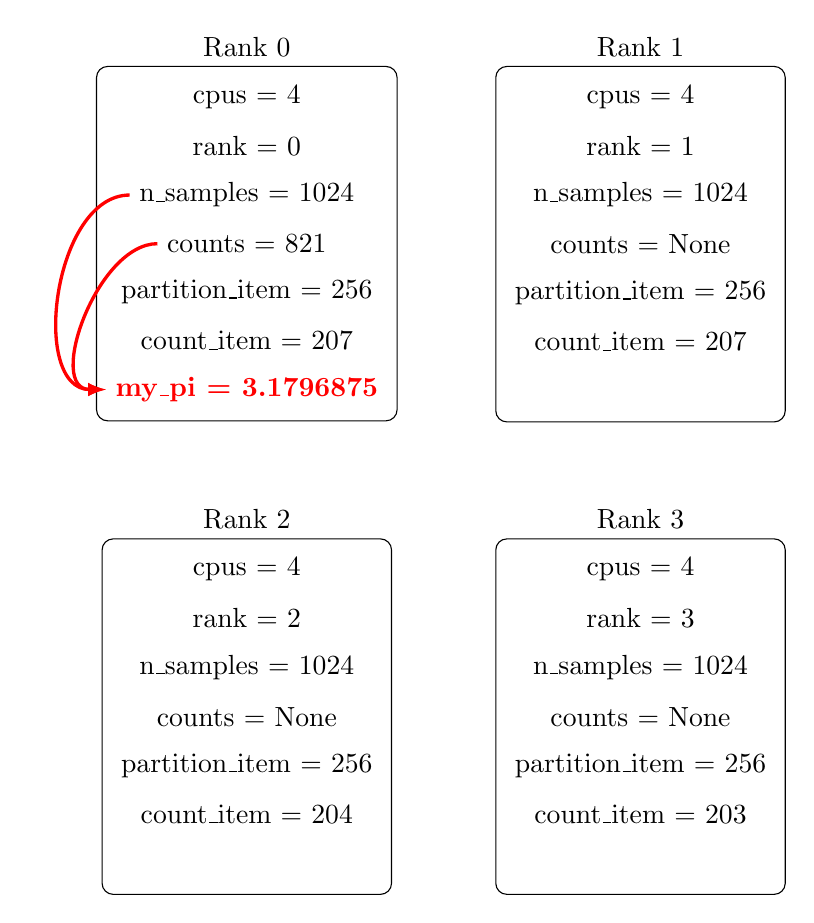
\begin{tikzpicture}
\tikzset{
  arrow/.style={
    >=latex
  },
  line/.style={
    draw,
    ->,
    very thick,
  },
  array/.style={
    draw,
    minimum size=0.5cm
  },
  new/.style={
    red,
    font=\bfseries
  },
  old/.style={
  }
}

% Globals
\newcommand{\cpus}{4}
\newcommand{\nsamples}{1024}
\newcommand{\partition}{256}

% Initialize
%\newcommand{\setstate}{
%\newcommand{\countstyle}{}
%\newcommand{\countszero}{0}
%\newcommand{\countsone}{0}
%\newcommand{\countstwo}{0}
%\newcommand{\countsthree}{0}
%\newcommand{\showpi}{\phantom}
%\newcommand{\pistyle}{}
%\newcommand{\pizero}{\partition}
%\newcommand{\pione}{\partition}
%\newcommand{\pitwo}{\partition}
%\newcommand{\pithree}{\partition}
%\newcommand{\showci}{\phantom}
%\newcommand{\cistyle}{}
%\newcommand{\cizero}{\countszero}
%\newcommand{\cione}{\countsone}
%\newcommand{\citwo}{\countstwo}
%\newcommand{\cithree}{\countsthree}
%\newcommand{\showmypizero}{\phantom}
%\newcommand{\showmypione}{\phantom}
%\newcommand{\showmypitwo}{\phantom}
%\newcommand{\showmypithree}{\phantom}
%\newcommand{\mypistyle}{}
%\newcommand{\mypizero}{None}
%\newcommand{\mypione}{None}
%\newcommand{\mypitwo}{None}
%\newcommand{\mypithree}{None}
%\newcommand{\drawarrows}{}
%}

% Calculate work to do
%\newcommand{\setstate}{
%\newcommand{\countstyle}{}
%\newcommand{\countszero}{None}
%\newcommand{\countsone}{None}
%\newcommand{\countstwo}{None}
%\newcommand{\countsthree}{None}
%\newcommand{\showpi}{}
%\newcommand{\pistyle}{new}
%\newcommand{\pizero}{\partition}
%\newcommand{\pione}{\partition}
%\newcommand{\pitwo}{\partition}
%\newcommand{\pithree}{\partition}
%\newcommand{\showci}{\phantom}
%\newcommand{\cistyle}{}
%\newcommand{\cizero}{\countszero}
%\newcommand{\cione}{\countsone}
%\newcommand{\citwo}{\countstwo}
%\newcommand{\cithree}{\countsthree}
%\newcommand{\showmypizero}{\phantom}
%\newcommand{\showmypione}{\phantom}
%\newcommand{\showmypitwo}{\phantom}
%\newcommand{\showmypithree}{\phantom}
%\newcommand{\mypizero}{None}
%\newcommand{\mypione}{None}
%\newcommand{\mypitwo}{None}
%\newcommand{\mypithree}{None}
%\newcommand{\mypistyle}{}
%\newcommand{\drawarrows}{}
%}

% Compute
%\newcommand{\setstate}{
%\newcommand{\countstyle}{}
%\newcommand{\countszero}{None}
%\newcommand{\countsone}{None}
%\newcommand{\countstwo}{None}
%\newcommand{\countsthree}{None}
%\newcommand{\showpi}{}
%\newcommand{\pistyle}{}
%\newcommand{\pizero}{\partition}
%\newcommand{\pione}{\partition}
%\newcommand{\pitwo}{\partition}
%\newcommand{\pithree}{\partition}
%\newcommand{\showci}{}
%\newcommand{\cistyle}{new}
%\newcommand{\cizero}{200}
%\newcommand{\cione}{207}
%\newcommand{\citwo}{204}
%\newcommand{\cithree}{203}
%\newcommand{\showmypizero}{\phantom}
%\newcommand{\showmypione}{\phantom}
%\newcommand{\showmypitwo}{\phantom}
%\newcommand{\showmypithree}{\phantom}
%\newcommand{\mypistyle}{}
%\newcommand{\mypizero}{None}
%\newcommand{\mypione}{None}
%\newcommand{\mypitwo}{None}
%\newcommand{\mypithree}{None}
%\newcommand{\drawarrows}{
%}
%}

% Reduce
%\newcommand{\setstate}{
%\newcommand{\countstyle}{new}
%\newcommand{\countszero}{821}
%\newcommand{\countsone}{None}
%\newcommand{\countstwo}{None}
%\newcommand{\countsthree}{None}
%\newcommand{\showpi}{}
%\newcommand{\pistyle}{}
%\newcommand{\pizero}{\partition}
%\newcommand{\pione}{\partition}
%\newcommand{\pitwo}{\partition}
%\newcommand{\pithree}{\partition}
%\newcommand{\showci}{}
%\newcommand{\cistyle}{}
%\newcommand{\cizero}{200}
%\newcommand{\cione}{207}
%\newcommand{\citwo}{204}
%\newcommand{\cithree}{203}
%\newcommand{\showmypizero}{\phantom}
%\newcommand{\showmypione}{\phantom}
%\newcommand{\showmypitwo}{\phantom}
%\newcommand{\showmypithree}{\phantom}
%\newcommand{\mypistyle}{}
%\newcommand{\mypizero}{None}
%\newcommand{\mypione}{None}
%\newcommand{\mypitwo}{None}
%\newcommand{\mypithree}{None}
%\newcommand{\drawarrows}{
%  \draw[red, line, arrow, out=180, in=0] (countitem0) to (counts0);
%  \draw[red, line, arrow, out=180, in=0] (countitem1) to (counts0);
%  \draw[red, line, arrow, out=180, in=0] (countitem2) to (counts0);
%  \draw[red, line, arrow, out=180, in=0] (countitem3) to (counts0);
%}
%}

% Finalize
\newcommand{\setstate}{
\newcommand{\countstyle}{}
\newcommand{\countszero}{821}
\newcommand{\countsone}{None}
\newcommand{\countstwo}{None}
\newcommand{\countsthree}{None}
\newcommand{\showpi}{}
\newcommand{\pistyle}{}
\newcommand{\pizero}{\partition}
\newcommand{\pione}{\partition}
\newcommand{\pitwo}{\partition}
\newcommand{\pithree}{\partition}
\newcommand{\showci}{}
\newcommand{\cistyle}{}
\newcommand{\cizero}{200}
\newcommand{\cione}{207}
\newcommand{\citwo}{204}
\newcommand{\cithree}{203}
\newcommand{\showmypizero}{}
\newcommand{\showmypione}{\phantom}
\newcommand{\showmypitwo}{\phantom}
\newcommand{\showmypithree}{\phantom}
\newcommand{\mypistyle}{new}
\newcommand{\mypizero}{3.1796875}
\newcommand{\mypione}{none}
\newcommand{\mypitwo}{none}
\newcommand{\mypithree}{none}
\newcommand{\drawarrows}{
  \draw[red, line, arrow, out=180, in=180] (counts0) to (mypi0);
  \draw[red, line, arrow, out=180, in=180] (nsamples0) to (mypi0);
}
}

\setstate
% Rank 0
% initial state:
% cpus = 4, rank = 0, n_samples = 1024,
% counts = None
% after calculation:
% partition_item = 256, count_item = 0
% after inside_circle(partition_item):
% count_item = something0
% after reduce:
% counts = something0 + something1 + something2 + something3
% my_pi = 4*sum(counts)/n_samples
\node (cpus0) [xshift=0 cm, yshift=6cm] {cpus = \cpus};
\node (rank0) [below=.1 cm of cpus0] {rank = 0};
\node (nsamples0) [below=.1 cm of rank0] {n\_samples = \nsamples};
\node (counts0) [below=.1 cm of nsamples0] {counts = \countszero};
\node (partitionitem0) [below=.1 cm of counts0, \pistyle] {\showpi{partition\_item = \pione}};
\node (countitem0) [below=.1 cm of partitionitem0, \cistyle] {\showci{count\_item = \cione}};
\node (mypi0) [below=.1 cm of countitem0, \mypistyle] {\showmypizero{my\_pi = \mypizero}};
\node (rank0t) [fit=(cpus0) (rank0) (nsamples0) (counts0) (partitionitem0) (countitem0) (mypi0), label=above:{Rank 0}, draw, rounded corners] {};


% Ranks 1,2,3
% initial state:
% cpus = 4, rank = rank, n_samples = 1024,
% counts = None
% after calculation:
% partition_item = 256, count_item = 0
% after inside_circle(partition_item):
% count_item = something1
\node (cpus2) [xshift=0 cm, yshift=0cm] {cpus = \cpus};
\node (rank2) [below=.1 cm of cpus2] {rank = 2};
\node (nsamples2) [below=.1 cm of rank2] {n\_samples = \nsamples};
\node (counts2) [below=.1 cm of nsamples2] {counts = \countstwo};
\node (partitionitem2) [below=.1 cm of counts2, \pistyle] {\showpi{partition\_item = \pitwo}};
\node (countitem2) [below=.1 cm of partitionitem2, \cistyle] {\showci{count\_item = \citwo}};
\node (mypi2) [below=.1 cm of countitem2, \mypistyle] {\showmypitwo{my\_pi = \mypitwo}};
\node (rank2t) [fit=(cpus2) (rank2) (nsamples2) (counts2) (partitionitem2) (countitem2) (mypi2), label=above:{Rank 2}, draw, rounded corners] {};


\node (cpus1) [xshift=5 cm, yshift=6cm] {cpus = \cpus};
\node (rank1) [below=.1 cm of cpus1] {rank = 1};
\node (nsamples1) [below=.1 cm of rank1] {n\_samples = \nsamples};
\node (counts1) [below=.1 cm of nsamples1] {counts = \countsone};
\node (partitionitem1) [below=.1 cm of counts1, \pistyle] {\showpi{partition\_item = \pione}};
\node (countitem1) [below=.1 cm of partitionitem1, \cistyle] {\showci{count\_item = \cione}};
\node (mypi1) [below=.1 cm of countitem1, \mypistyle] {\showmypione{my\_pi = \mypione}};
\node (rank1t) [fit=(cpus1) (rank1) (nsamples1) (counts1) (partitionitem1) (countitem1) (mypi1), label=above:{Rank 1}, draw, rounded corners] {};

\node (cpus3) [xshift=5 cm, yshift=0cm] {cpus = \cpus};
\node (rank3) [below=.1 cm of cpus3] {rank = 3};
\node (nsamples3) [below=.1 cm of rank3] {n\_samples = \nsamples};
\node (counts3) [below=.1 cm of nsamples3] {counts = \countsthree};
\node (partitionitem3) [below=.1 cm of counts3, \pistyle] {\showpi{partition\_item = \pithree}};
\node (countitem3) [below=.1 cm of partitionitem3, \cistyle] {\showci{count\_item = \cithree}};
\node (mypi3) [below=.1 cm of countitem3, \mypistyle] {\showmypithree{my\_pi = \mypithree}};
\node (rank3t) [fit=(cpus3) (rank3) (nsamples3) (counts3) (partitionitem3) (countitem3) (mypi3), label=above:{Rank 3}, draw, rounded corners] {};


\drawarrows

\end{tikzpicture}

\end{document}
